\documentclass[tikz,border=10pt]{standalone}
% Scale s = 0.012719 cm/px, centred on ink bbox centre (352, 159.5); y flipped
\begin{document}
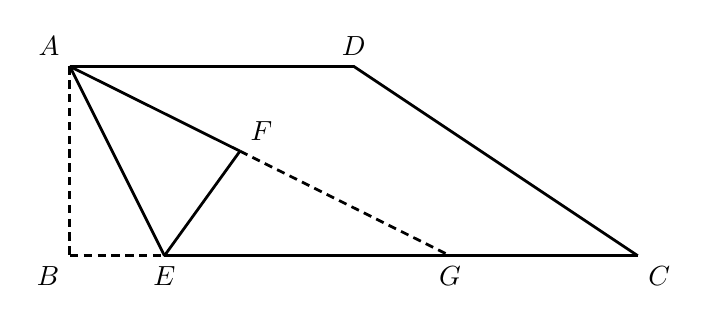
\begin{tikzpicture}[line width=1.0pt, line join=round, font=\fontsize{10}{12}\selectfont]
% Named coordinates (cm)
\coordinate (A) at (-3.606,1.202);
\coordinate (B) at (-3.606,-1.202);
\coordinate (C) at (3.606,-1.202);
\coordinate (D) at (0,1.202);
\coordinate (E) at (-2.405,-1.202);
\coordinate (F) at (-1.446,0.126);
% G: intersection of line AF with base y=254 px (448,254) px
\coordinate (G) at (1.221,-1.202);

% Solid edges
\draw (A) -- (D) -- (C);      % top edge and right side
\draw (E) -- (C);             % base, solid part
\draw (A) -- (E);
\draw (F) -- (E);
\draw (A) -- (F);

% Dashed edges
\draw[dash pattern=on 3pt off 2pt] (A) -- (B);
\draw[dash pattern=on 3pt off 2pt] (B) -- (E);
\draw[dash pattern=on 3pt off 2pt] (F) -- (G);  % continuation of AF to base

% Labels
\node[above left]  at (A) {$A$};
\node[below left]  at (B) {$B$};
\node[below right] at (C) {$C$};
\node[above]       at (D) {$D$};
\node[below]       at (E) {$E$};
\node[above right] at (F) {$F$};
\node[below]       at (G) {$G$};
\end{tikzpicture}
\end{document}